

\chapter{Background} % Main chapter title

\textcolor{Cite the references you used at appropriate places}
%----------------------------------------------------------------------------------------

% Define some commands to keep the formatting separated from the content 
\newcommand{\keyword}[1]{\textbf{#1}}
\newcommand{\tabhead}[1]{\textbf{#1}}
\newcommand{\code}[1]{\texttt{#1}}
\newcommand{\file}[1]{\texttt{\bfseries#1}}
\newcommand{\option}[1]{\texttt{\itshape#1}}

%----------------------------------------------------------------------------------------
\section{Cryptosystem}
\hspace{10mm} 
With the progress of modern informatics taking over and advances of technology the topic of security is more relevant than ever. Communications, transactions and exchanges in information are advancing each day, which is why the use of cryptography is crucial to help ensure security in the processes. Companies are more willing to invest in security in terms of means of transmitting classified data. This could be anything from personal data like credit card information to codes and strategies that a corporation wants to keep hidden. To achieve this,  In other words, it is the science of keeping information hidden and secure from unintended audiences. A more formal definition of a cryptosystem is presented.

\begin{definition}
    A \ita{cryptosystem} (or \ita{cipher}) can be defined as a quintuple (P, C, K, E, D)  where: 
        \begin{itemize}
            \item P is the set of plaintexts
            \item C is the set of ciphertexts
            \item K is the set of keys
            \item E: K $\times$ P $\rightarrow$ C is the encryption function 
            \item D: K $\times$ C $\rightarrow$ P is the decryption function 
        \end{itemize}
\end{definition}

\hspace{10mm}  Here, the original message that is meant to be sent is called the plaintext. This will be encoded as a ciphertext and at most times will be written in the same alphabet as the plaintext. The plaintext and the ciphertext will also contain the same number of characters. 

\section{Message sending process}

\hspace{10mm} The process of converting a plaintext to ciphertext is called encryption, and the inverse process is called decryption. The basic process of sending a message is described below involving three people, Alice, Bob, and Eve:

\begin{itemize}

\item Alice wants to send a message called plaintext to Bob
\item For Eve to not find out about the message, Alice will encrypt the plaintext into a ciphertext. This is done using an encryption key.
\item Bob receives the ciphertext and decrypts it using a decryption key and can read the plaintext.
\item Eve is not able to decrypt the messege without a  decryption key, so the messege between Alice and Bob stays secure

\end{itemize}

\section{Introduction to Elliptic Curves}


\hspace{10mm}  Modern cryptography uses algorithms and secret keys in order to encrypt and decrypt data and focuses mostly on the secrecy of the keys than the secrecy of the encryption method. Many cryptosystems have been proposed in order to provide the most optimal secrecy and integrity to data, as well as anonymity to the users. One of these methods is the use of elliptic curves.

\begin{definition}
 Let $K$ be a field of characteristic $\neq 2, 3$, and let $x^3 + ax + b$ (where $a, b \in K$) be a cubic polynomial with no multiple roots. An \textit{elliptic curve} over K is the set of all points $(x, y)$ with $x, y \in K$ which satisfy the
equation

\begin{equation}
y^2 = x^3 + ax + b
\end{equation}

together with a single element denoted $\mathcal{O}$ and called the \textit{Point at Infinity}.\footnote{Koblitz, N. (1994)}
\end{definition}
 
\begin{figure}
    \centering
    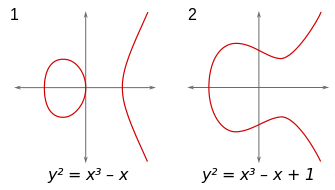
\includegraphics{Figures/ECClines-3.jpg}
    \caption{}
    \label{fig:my_label}
\end{figure}

We will denote the elliptic curve over $K$, as the set $E(K)$ such that
\begin{equation}
    E(K)=\{(x,y) \in K^2 | y^2=x^3+ax+b, a,b \in K\} \cup \{\mathcal{O}\}
\end{equation}


\hspace{10mm} The use of elliptic curves has risen because it provides equivalent security compared to other systems like RSA (Rivest-Shamir-Adleman), but with the use of fewer bits. A typical Elliptic Curve Cryptosystem key size of 256 bits has the same security as an RSA key of 3072 bits. So, on the long run, RSA keys have to get exponentially large to provide equivalent security compared to the fewer bits that the Elliptic Curves Cryptosystem can provide. Another reason for their use is that it becomes an alternative in case that a major weakness is RSA is found. 

\hspace{10mm}  Other reasons for why this cryptosystem has been beneficial is because it is faster than systems like RSA. This is because of the use of smaller keys, which means that less data will be transmitted from server to client. Also, it will take less processing power (CPU) which will again, bring faster responses. \footnote{Thayer, W. (2015, April 04)}


